% Chapter 8

\chapter{Flow Chart}
\label{Chapter8}

Once interrupt source triggers the interrupt, it then goes to gateway and then gateway will request that interrupt to PLIC Core which is shown in the Figure \ref{fig:flow_chart}. 

\par
After the interrupt is requested to PLIC core, it will then \textbf{alert/notify} target(s). Now the important step comes, after the target has received the interrupt, it will send a signal back to PLIC core that this interrupt is claimed (Also the claim ID). Receiving the claim from target, PLIC will send claim response that this interrupt should be serviced or not. Then the interrupt handler services the that particular interrupt. 


\begin{figure}[h]
  \centering
  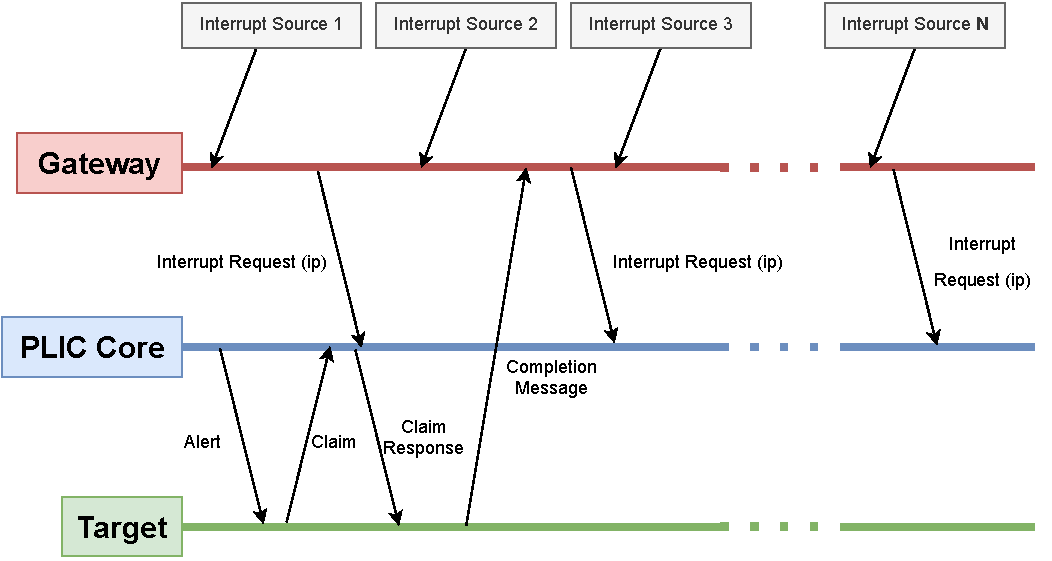
\includegraphics[width=1\textwidth]{F:/FYP/flow_chart.pdf}
  \caption{Flow Chart.}
  \label{fig:flow_chart}
\end{figure}


Finally, the interrupt completion message will be sent to gateway that this interrupt is completed and no need to send any other interrupt from that source. So is the case with all other pending interrupts from other sources.

